\subsection{Sensor and Circuit Design for Torque Measurements}
\label{sec:circuitDesignNsensor}

The sensor was paired with an amplifier circuit, made following the ideas described in Chiu \textit{et al.}(2016)\cite{Chiu2016CharacterizationOA}. For our use case the sensor was fabricated from different non-magnetic materials to assess which would make the better sensor. 

%This work predates this document and exists only as lab-notebook entries and circuit sketches. Relevant portions are included both as documentation and as the starting point for the retesting and characterization carried out.

%\subsubsection{Sensor Design}
The sensor is formed by the beam and a pair of $\text{OMEGA}^{\text{\tiny \textregistered}}$ precision strain gauges (SGD-3/350-LY11) \cite{omega_SGD_LINEAR1_AXIS}. These strain gauges were epoxied on opposite sides of the rod around 3 to 5 cm from its end, depicted in Figure \ref{fig:cantilever3d}. The strain gauges are part of a Half-Wheatstone bridge configuration and are connected to the circuit with soldered jumper wires.%, described in Section \ref{sec:circuit}. 

\begin{figure}[hbt!]%{R}{0.48\textwidth}
	\centering
	%\vspace{-30pt}
	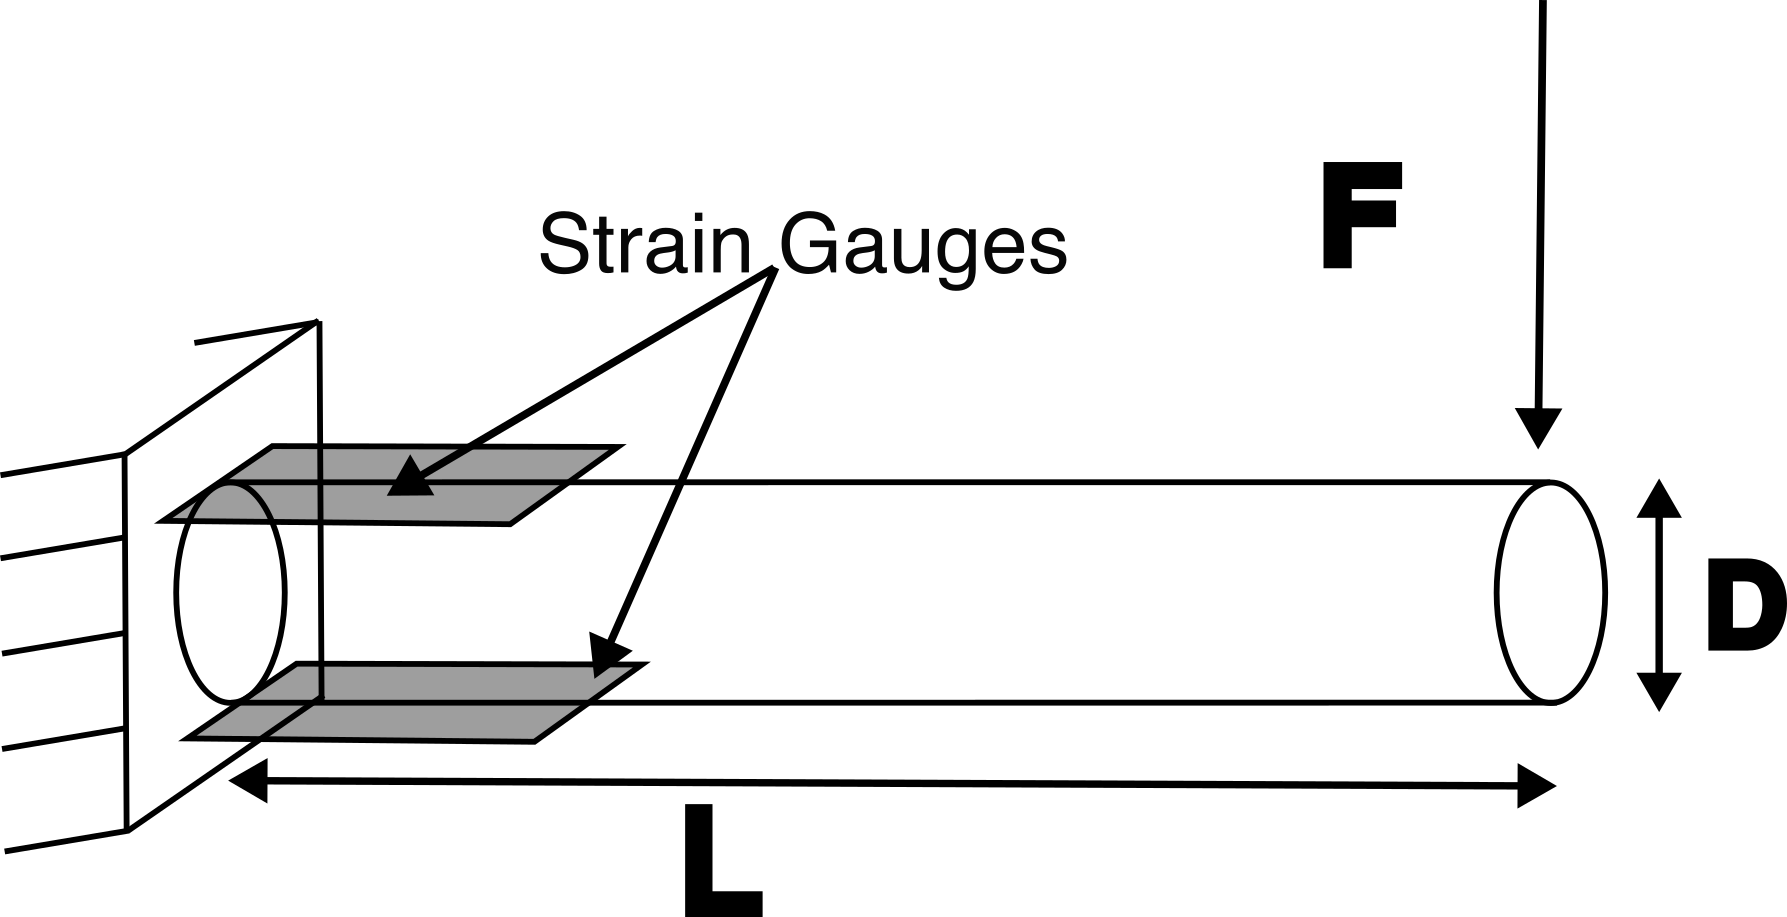
\includegraphics[width=0.48\textwidth]{Assets/cantilever3d.png}
	\caption{Cantilever setup showing the fixed cylinder and strain gauges ''sandwiching" the rod at its base.}
	\label{fig:cantilever3d}
	%\vspace{-10pt}
\end{figure}

Figure \ref{fig:rods} shows a sample set of seven beam force sensors which were produced in the laboratory. The beam materials included glass, aluminum, titanium and two types of plastic. Table \ref{tab:rods} summarizes their characteristics. They were made of similar sizes to test repeatability. %Two of the seven available sensors were found to be irreparably damaged, so no further measurements were possible on them.

\begin{figure}[hbt!]
	\centering
	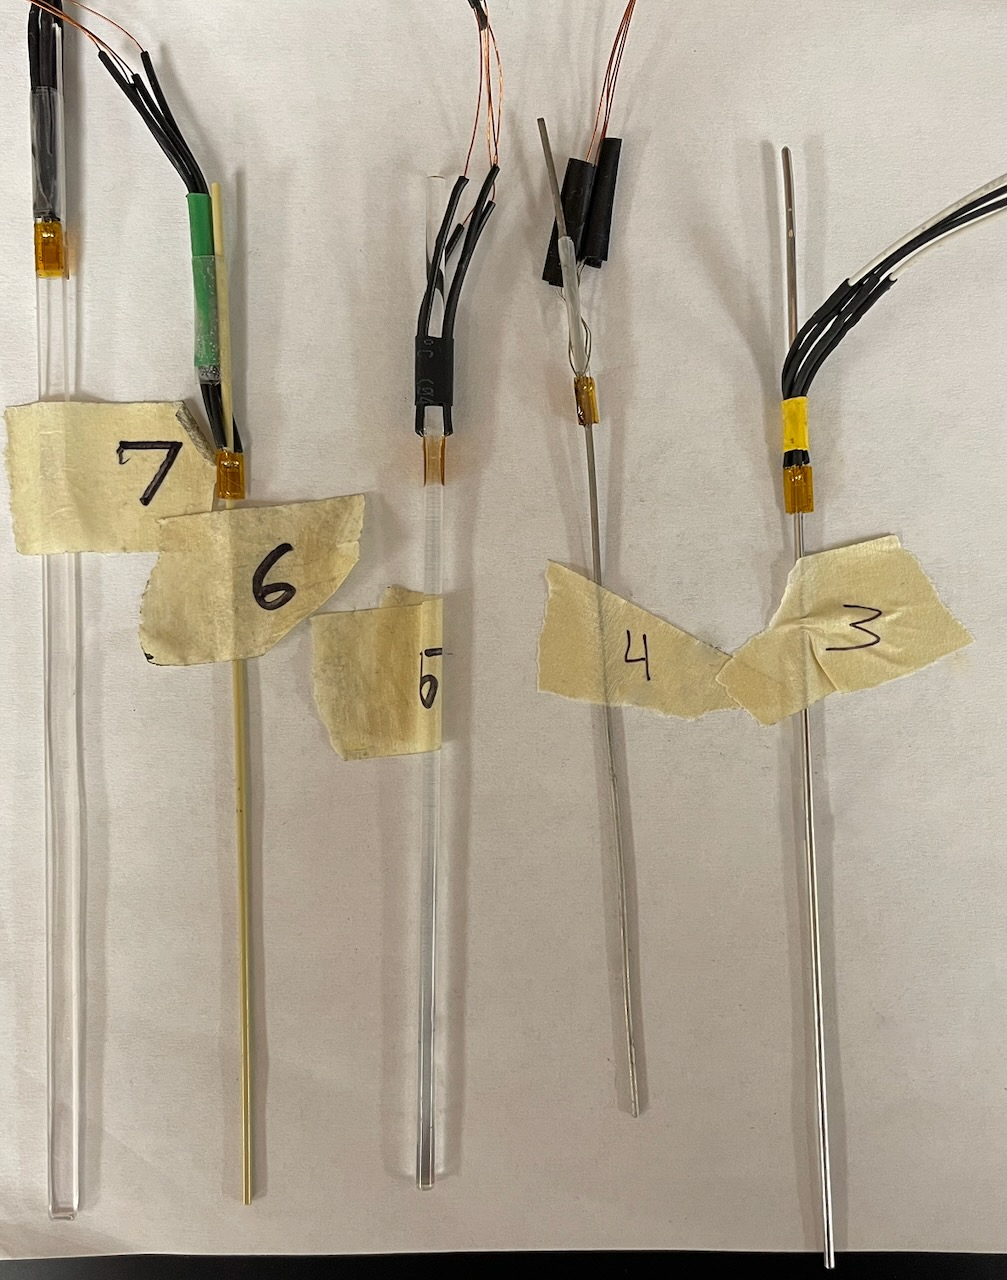
\includegraphics[width=0.4\textwidth]{Assets/rods.png}
	\caption[Rod used in the experiment]{Rods fabricated during the torque experiment design. From left to right, (7) Clear Plastic, (6) Yellow plastic, (5) Glass, (4) Titanium, (3) Aluminum}
	\label{fig:rods}
\end{figure}

\begin{table}[htb!]
	\centering
	\caption{Characteristics of the sensor rods.}
	\label{tab:rods}
	\begin{tabular}{llll}
		Rod ID & Material & Diameter (mm) & Length (mm) \\
		\hline
		1 & Aluminum (Al)& 1.6 & 145  \\
		2 & Al & 1.6 & 182 \\
		3 & Al & 1.6 & 182  \\
		4 &  Titanium & 1.02 & 220 \\
		5 &  glass & 3.2 & 166.00 \\
		6 & yellow plastic & 1.6 & 220 \\ 
		7 &  clear plastic & 2.9 & 180 \\
	\end{tabular}
	
\end{table}
%\footnotetext[1]{This rod was originally stored on a spool and had to be straightened manually. That process introduced micro-cracks, so the material no longer behaved elastically and deviated from Hooke’s law.}
%\footnotetext[2]{This rod was discovered broken in the circuitry and was noticeably bent, indicating the need for full refabrication.}
On the other hand, the circuit prototype of Chiu \textit{et al.}(2016), shown in Figure \ref{fig:torqueCircuit} hav four main sections: the Wheatstone bridge, the amplifier, a low pass filter and the ground offset potentiometers. The potentiometers were an addition to the original design. A Kirchhoff analysis for the first two sections yielded the transmission function.

\begin{figure}[htb!]
	\centering
	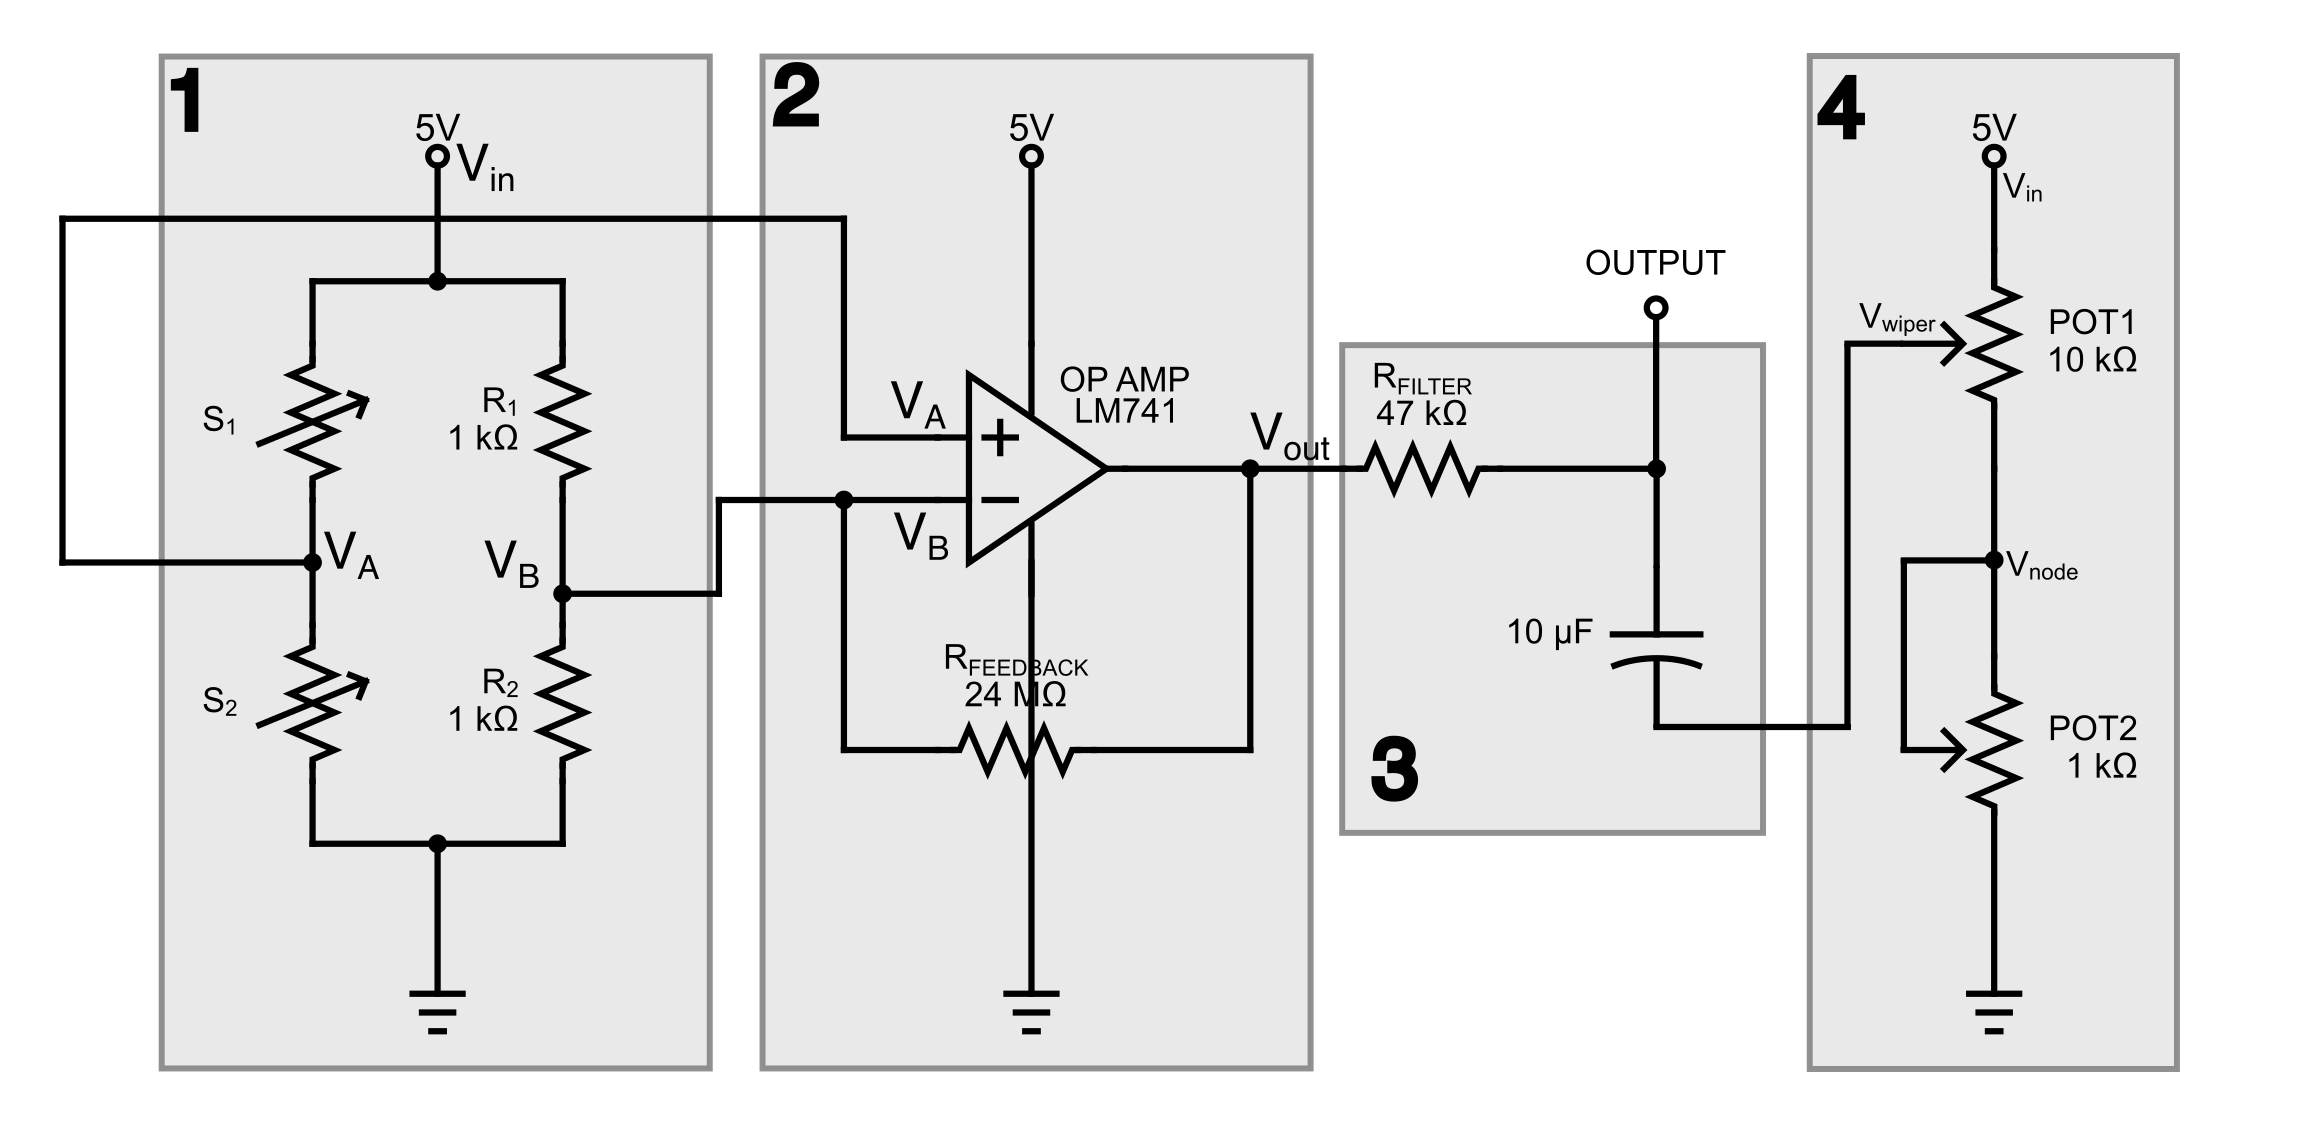
\includegraphics[width=\textwidth]{Assets/circuit.png}
	\caption[Torque‐measurement circuit based on Chiu 2016]{Circuit developed for the torque measurement setup, following the design principles of Chiu \textit{et al.} (2016)\cite{Chiu2016CharacterizationOA}. Features include, 1. Half Wheastone Bridge Strain Gauge, 2. Amplifier, 3. Low-pass filter, 4. Coarse–fine adjustable reference network.}
	\label{fig:torqueCircuit}
\end{figure}

\begin{equation}
	\label{eq:kirchov12}
	\frac{V_{out}}{V_{in}} = \frac{R_{FEEDBACK}}{R} \frac{S_2 - S_1}{S_2 + S_1} + \frac{S_2}{S_2 + S_1},
\end{equation}

\noindent where $R = R_1 = R_2$, $S_1$ and $S_2$ are the strain gauge variable resistance input (or signal coming from the sensor) and $R_{FEEDBACK}$ is the feedback loop needed for amplification. The output voltage of the circuit is driven by the relative difference between the two strain gauges compared to their total resistance. The operational amplifier multiplies this small imbalance by the gain factor $\frac{R_{FEEDBACK}}{R}$. The bridge sets a baseline through the voltage division
$
\frac{S_2}{S_2 + S_1},
$
whereas the amplified differential term
$
\frac{S_2 - S_1}{S_2 + S_1}
$
determines the sensitivity of the circuit to strain. For the complete derivation see Appendix \ref{app:Kirchhoff}.

%\subsection*{Low–Pass Filtering and Reference-Voltage Behavior}

After the instrumentation–amplifier stage, the output passes through a first–order RC low–pass filter composed of a \(47~\text{k}\Omega\) resistor in series with a \(10~\mu\text{F}\) capacitor to ground, as in Figure \ref{fig:torqueCircuit} part 3. The time constant is then $\tau= 0.47~\text{s}$, yielding a $0.33~\text{Hz}$ cutoff frequency. Finally, a first–order system with this time constant has a \(10\rightarrow 90\%\) rise time of approximately $1.03~\text{s}$. In other words, whatever the Wheatstone–op-amp transfer function generates, this RC stage only slows its dynamics rather than altering its steady–state gain. It suppresses high–frequency noise from the strain gauge bridge and smooths fast fluctuations that the rod could not physically produce.


%\subsection*{Reference-Voltage Control Using Coarse–Fine Potentiometers}

In part 4 of Figure \ref{fig:torqueCircuit}, the DC reference entering the filter is set by the two potentiometers (analyzed in Appendix~\ref{app:pots}).
Both potentiometers are connected in series, forming a programmable voltage divider from 0 to 5V. The capacitor of RC network simply charges toward whichever reference these pots define. From the voltage-divider derivation in Appendix~\ref{app:pots}, the node voltage obeys

\begin{equation}
	\label{eq:voltageDivider}
	V_{\text{ref}} =
	V_{\text{in}}
	\frac{R_{2}}{R_{1}+R_{2}},
\end{equation}


\noindent so sweeping the fine pot moves \(R_{2}\) over a narrow range(\(\sim 0\)–\(1~\text{k}\Omega\)), which shifts the reference only within a small, controllable window. The coarse pot changes the large \(R_{1}\) segment (\(\sim 10~\text{k}\Omega\)), expanding or collapsing the overall span. 

Understanding both the strain at the sensor and the electrical physics of the circuit enables identification of the measurement device's capabilities. We now proceed to validate our sensor construction against the reference provided by Chiu \textit{et al.} (2016)\cite{Chiu2016CharacterizationOA}.

\subsubsection{Smallest measurable torque}
\label{sec:SmallTorque}

\begin{wrapfigure}[7]{R}{0.38\textwidth}
	\centering
	%\vspace{-5pt}
	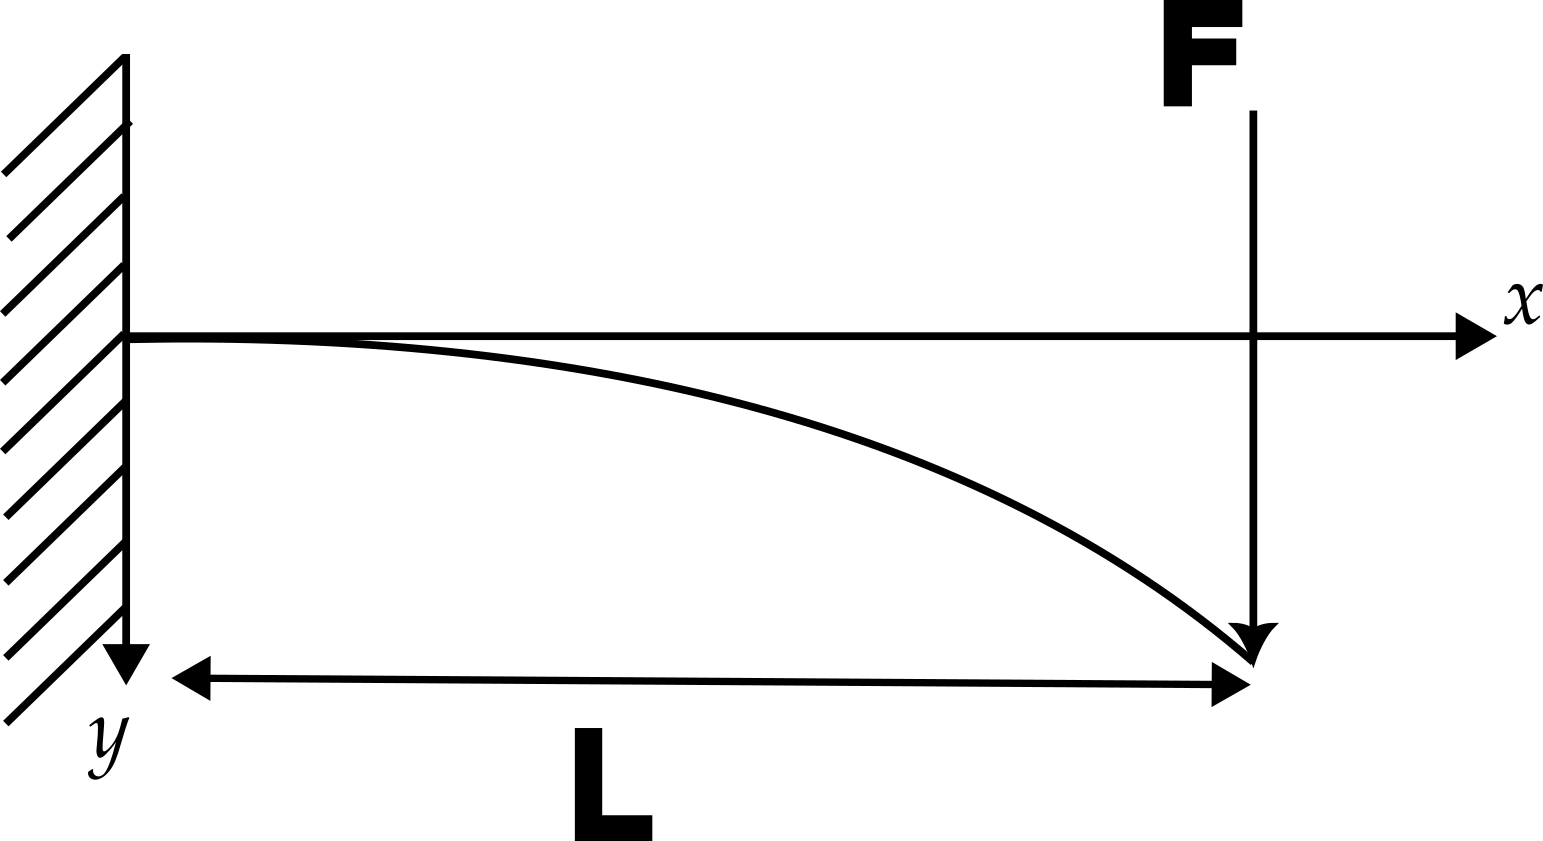
\includegraphics[width=\linewidth]{Assets/cantileverDiagram.png}
	\caption{Cantilever Beam of length L with concentrated load F at the free end.}
	\label{fig:cantileverDiagram}
	%\vspace{10pt}
\end{wrapfigure}

For torque measurements, the sensitivity of cantilever-based torque sensors is determined primarily by the relationship between the applied tip load and the strain induced at the fixed end of the beam. Figure \ref{fig:cantileverDiagram} shows a diagram for a thin cylindrical beam of length $L$ fixed at one end and subjected to a transverse point load $F$ at the free tip. Classical beam theory \cite{hibbeler2016mechanics,Chiu2016CharacterizationOA} gives the maximum surface strain as

\begin{equation}
	\epsilon = \frac{32 F L}{\pi E D^3},
	\label{eq:strain_beam}
\end{equation}

\noindent where $D$ is the diameter, and $E$ is the Young’s modulus. This relationship indicates that the strain is inversely related to the Young's modulus and the cube of the diameter and directly proportional to beam length. As a result, longer and thinner rods increase the observable signal by producing greater strain for the same applied force.  

Following the geometry used by Chiu \textit{et al.} (2016)\cite{Chiu2016CharacterizationOA}, a wire of $L = 69.85\,{mm}$ and $D = 0.64\,{mm}$ fabricated from Nitinol ($E = 66.2\,{GPa}$) achieved an empirical detection limit of $0.49\,{mN}$. Using Equation~\ref{eq:strain_beam}, this translates to a geometric sensitivity factor on the order of $L/D^3 \approx 2.66\times10^8\,{m^{-2}}$, isolating the geometry-dependent amplification of strain and therefore serving as a design metric for mechanical sensitivity. 

A similar configuration can, in principle, achieve micro-Newton sensitivity when paired with a low-noise amplification circuit, provided the strain gauge and readout maintain linear response and the system noise floor remains below the equivalent strain corresponding to the smallest measurable force.

%\subsection{Conversion from Strain to Electrical Signal}

In the actual implementation, a metallic foil strain gauge bonded to the beam surface, which its position is shown in Figure \ref{fig:cantilever3d} and \ref{fig:rods}, converts the mechanical strain into a measurable change in electrical resistance. For small elastic deformations, the fractional change in resistance is linearly related to strain through the gauge factor $G_F$ \cite{fraden2016handbook,MicroMeasurements,OmegaSG},

\begin{equation}
	\frac{\Delta R}{R} = {G_F} \, \epsilon,
	\label{eq:resistance_strain}
\end{equation}

\noindent
where $G_F$ is typically in the range of $2.0$–$2.2$ for constant foil gauges. 
Combining Equations~\ref{eq:strain_beam} and \ref{eq:resistance_strain} gives the total resistance change due to an applied tip force.

\begin{equation}
	\Delta R = R_0 \, {G_F} \, \frac{32 F L}{\pi E D^3}.
	\label{eq:resistance_force}
\end{equation}

\noindent
This resistance change is converted to a differential voltage when the gauge is part of a Wheatstone bridge circuit. For a half-bridge configuration, where two active strain gauges form adjacent arms of the bridge, the small-signal output voltage under excitation $V_{exc}$ is approximately \cite{fraden2016handbook,NI_AN078_1998}

\begin{equation}
	V_{out} \approx \frac{V_{exc}}{2} \, G_F \, \epsilon,
	\label{eq:bridge_output}
\end{equation}

\noindent assuming perfect linearity, little temperature drift, and perfect bridge balancing. The direct proportionality between applied force and bridge voltage may be obtained by combining Equation~\ref{eq:strain_beam} into \ref{eq:bridge_output},

\begin{equation}
	V_{out} = 16 \, G_F \, V_{exc} \frac{L}{\pi E D^3} \, F.
	\label{eq:force_to_voltage}
\end{equation}

In practice, the smallest detectable force is governed by the combined noise of the gauge, bridge, and amplifier system. 
If the noise-equivalent output voltage $V_{noise}$ corresponds to a minimum detectable strain $\epsilon_{min} = \frac{2V_{noise}}{(V_{exc} G_F G)}$, then the force detection limit follows from Equation~\ref{eq:strain_beam} as

\begin{equation}
	F_{min} = \frac{\pi E D^3}{32 L} \, \epsilon_{min}.
	\label{eq:force_limit}
\end{equation}

Theoretically, the sensor can resolve forces in the milli-Newton range by optimizing the geometric ratio $L/D^3$, minimizing circuit noise, and selecting materials with moderate elastic modulus (e.g., aluminum or Nitinol). Using the parameters reported by Chiu \textit{et al.} (2016), such as bridge noise of $\sigma_V = 3$ mV and gain of 100, Equation~\ref{eq:force_limit} yields a minimum detectable force of $F_{\min} = 0.161~$mN (see Appendix~\ref{app:smallestTorque} for sample calculations). This theoretical floor assumes ideal amplification and no parasitic noise; in practice, real circuit noise raises the empirical detection limit, as Chiu et al. report 0.49 mN approximately three times above the theoretical floor of 0.161 mN, consistent with real-world imperfect conditions.

For the present design, the limit of detection is expressed in terms of torque. This is obtained by multiplying the minimum detectable force by the transfer arm length $r$, as described in Sections~\ref{sec:TorqMeasureApp} and \ref{sec:circuitDesignNsensor}. Using the parameters summarized in Table~\ref{tab:sensor_params}, the minimum detectable force is $\approx$ 0.094 mN, corresponding to a torque resolution of $\sigma_{\tau} = 4.70~\mu$N$\cdot$m under ideal conditions. The experimental test results for glass and plastic are reported in Appendix~\ref{app:addRes_senCal} with aluminum results on Section \ref{sec:restorqueLab}, both following the calibration methodology of Section~\ref{sec:sensorCal}.

\begin{table}[hbt!]
	\centering
	\caption{Summary of the sensor and circuit parameters used for force and torque resolution estimation. Values are set for an aluminum-based sensor, paired with the circuit explained in Section \ref{sec:circuitDesignNsensor}}
	\label{tab:sensor_params}
	\begin{tabular}{|l|c|c|}
		\hline
		Parameter & Symbol & Value \\
		\hline
		Young's modulus & $E$ & 68 GPa \\
		Wire diameter & $d$ & 1.6 mm \\
		Beam length & $L$ & 182 mm \\
		\hline
		Bridge noise & $\sigma_V$ & 0.0005 V \\
		Excitation voltage & $V_{\text{exc}}$ & 5 V \\
		Gauge factor & $G_F$ & 2 \\
		Gain & $G$ & 160 \\
		\hline \hline
		Min. Force & $F_min$ & 0.094 mN \\
		Min. Torque & $\tau_min$ & 4.70~$\mu$ N$\cdot$m  \\
		\hline
	\end{tabular}
\end{table}

These restrictions can be decreased by averaging ($\sigma$ scales as $1/\sqrt{N}$), by increasing mechanical leverage (slope grows almost linearly with cantilever length), or by enhancing the bridge/amplifier noise performance. For quasi-static measurements, the limits of detection may be moved from tens of mg into the single-mg or sub-mg range using a combination technique (longer/thinner cantilever + averaging + low-noise amplifier); dynamic measurements will be constrained by bandwidth and 1/f drift.

Now we turn to experimentally quantifying the relationship between applied force (or weight) and the voltage output from our system.

\subsection{Sensor Calibration}
\label{sec:sensorCal}

Prior to any torque measurement, each sensor or rod from Table \ref{tab:rods} was tested or calibrated to accomplish two things: ensure the use of the most sensitive sensor and to acquire the conversion factor or slope of voltage to weight. Additionally, the orientation and position of the rods was tested to ensure optimal values on these parameters for torque measurements.

%include scale like calibration and boats, point to graphs on the appendix
For calibration in the lab, the sensor was set in a cantilever position as shown in Figure \ref{fig:boat}, so the bar faces horizontally and a small cone-shaped basket made out of tape was attached to hold increments of water. Water was added in $\mu$L increments (equivalent to milligrams) simulating torque loads from 0 to 800 mg. Initial increments of 10 to 200 $\mu $L covered the expected force range of epicardial leads weight, followed by additional 50 $\mu L$ increments to demonstrate linearity and sensor stability.

\begin{figure}[htb!]
	\centering
	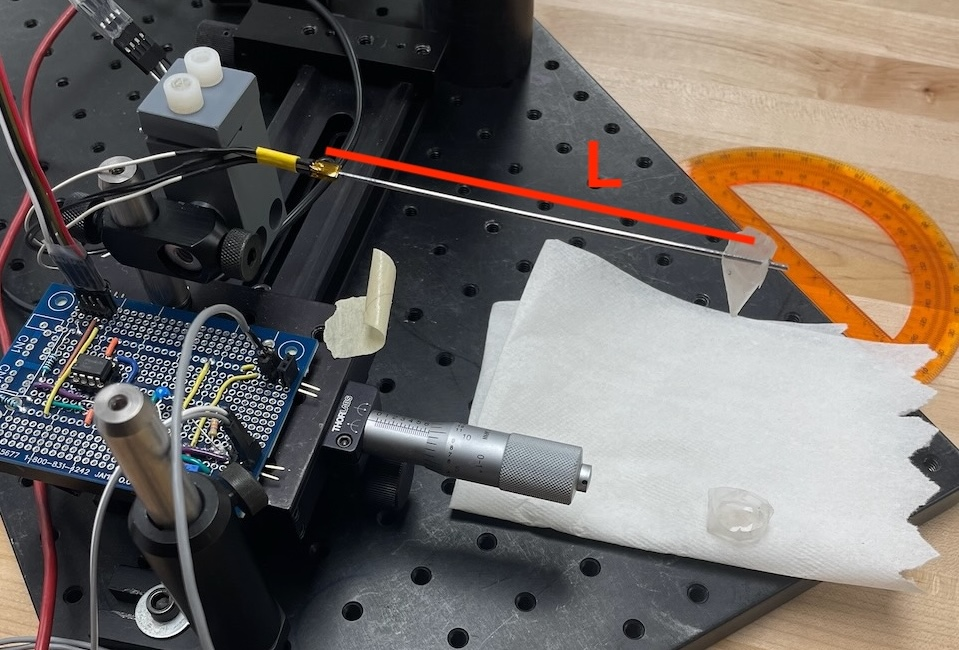
\includegraphics[width=0.6\textwidth]{Assets/boatSetupL.jpeg}
	\caption[Cantilever setup]{Circuit and sensor. The sensor was clamped with a custom made \gls{pvc} holder to act as a cantilever beam. A weigh boat at length $L$ was added, then a pipette was used to add water and calibrate voltage changes with weight.}
	\label{fig:boat}
\end{figure}

The sensor voltage vs. water mass was plotted and fit to a line to determine the calibration constant. This was done using python \texttt{Pandas} library in a Jupyter notebook and is publicly available \cite{juarezluna2025mrisafety}. This determine the signal resolution. The system is linearly calibrated by applying known weights to the free end of the cantilever, yielding the expected relationship

\begin{equation}
	\Delta V = k \Delta W
	\label{eq:torqueCal}
\end{equation}

\noindent where k, the slope of fit, is the calibration factor between voltage change ($\Delta V$) into the corresponding change in applied force ($\Delta W$ Weight).

%can be found, see Section \ref{sec:calResult}.

Then, in order to find the best position for sensor we set the following experiment, a set of neodymium magnets were aligned to the ceramic bearing to get a static magnetic field, and a platform angled at 45$^\circ$ carried the sensor as we moved it inwards. From section \ref{sec:torqueBG}, it was shown that the maximum torque appears at this angle. Then we tested for the optimal length ($L$) and position from the center ($r$) as shown in Figure \ref{fig:parameters}. This process was repeated to find the sweet spot on distance from the center up to a 100 mm radius and the best height was tested to different lengths along the rod sensor. 

\FloatBarrier